\documentclass[]{interact}

\usepackage{epstopdf} % To incorporate .eps illustrations using PDFLaTeX, etc.
\usepackage[caption=false]{subfig} % Support for small, `sub' figures and tables
%\usepackage[nolists,tablesfirst]{endfloat}% To `separate' figures and tables from text if required
%\usepackage[doublespacing]{setspace}% To produce a `double spaced' document if required
%\setlength\parindent{24pt}% To increase paragraph indentation when line spacing is doubled

\usepackage{amsmath}
\usepackage{amssymb}
\usepackage{algorithm}
\usepackage{algpseudocode} 
\usepackage{float}

\usepackage[numbers,sort&compress]{natbib} % Citation support using natbib.sty
\bibpunct[, ]{[}{]}{,}{n}{,}{,} % Citation support using natbib.sty
\renewcommand\bibfont{\fontsize{10}{12}\selectfont} % Bibliography support using natbib.sty
\makeatletter % @ becomes a letter
\def\NAT@def@citea{\def\@citea{\NAT@separator}} % Suppress spaces between citations using natbib.sty
\makeatother % @ becomes a symbol again

\theoremstyle{plain} % Theorem-like structures provided by amsthm.sty
\newtheorem{theorem}{Theorem}[section]
\newtheorem{lemma}[theorem]{Lemma}
\newtheorem{corollary}[theorem]{Corollary}
\newtheorem{proposition}[theorem]{Proposition}

\theoremstyle{definition}
\newtheorem{definition}[theorem]{Definition}
\newtheorem{example}[theorem]{Example}

\theoremstyle{remark}
\newtheorem{remark}{Remark}
\newtheorem{notation}{Notation}

\begin{document}

\articletype{} % Specify the article type or omit as appropriate

\title{Comparing the Performance Between Genetic and Clonal Selection Algorithm with Trivial Self-Driving Mechanism}

\author{
\name{Yejun Chang (Andrew)}
\affil{Henry M. Gunn High School}
}

\maketitle

\begin{abstract}
The rise in popularity of machine learning incited engineers to ponder ways that machines can self-learn without explicit programming of instructions. The paper compares the efficiency of genetic and clonal selection algorithm in a simple problem of navigating a car around the track. By assessing the efficiency, this paper analyzes how clonal selection algorithm can aid with machine learning problems and the inspirations we can take from the human immune system. A total of five different selection mechanisms were tested on a track with various widths and curves, and clonal selection algorithm was determined to be faster on average than genetic algorithms.
\end{abstract}

\begin{keywords}
artificial immune system; clonal selection algorithm; evolutionary algorithm; genetic algorithm; neural network; self driving;
\end{keywords}

\section{Introduction}

Humans are continuously inspired by the natural world, and computer algorithms are no exception to this everlasting trend. The rise of big data and smart systems in recent years has led software engineers to seek efficient machine learning algorithms, and many have caught interest in developing algorithms around biological ideas. Neural networks are currently at the center of this practice in order to emulate the unpredictable nature of a human brain for computers. One area that has been increasing in popularity in recent years is \textit{artificial immune system}. Inspired by the way our body fights the invading pathogens, artificial immune system emulates such process and aims solve complex machine learning problems.

In this paper, we will review the foundations of genetic and clonal selection algorithms and test how each performs in a machine learning problem of navigating a car around the track. Genetic algorithm will be divided into its own sub-categories by giving three variations to its selection operator. The goal is to assess the efficiency of each algorithms, analyze the benefits and drawbacks, and understand their differences and implications. Our analysis will be centered around the clonal selection algorithm and how artificial immune systems can fair in the field of machine learning.

\section{Background}

\subsection{Genetic Algorithm}
Genetic algorithm is a searching or an optimization algorithm inspired by Charles Darwin's biological evolutionary theory based on natural selection where the fittest individual survives and passes on the genes to its offspring. Similarly, genes are encoded accordingly to a particular problem in a genetic algorithm. Often structured with an array-like nucleic acids in a DNA strand, these genes determine an individual's behavior and thus its fitness. Those with higher fitness are then selected to create a subsequent generation with higher average fitness value. During this process, genetic recombination and mutation are performed to ensure variation in the population. By repeating these steps over multiple generations, the population can converge to a desired solution. A population is considered to have converged if at least 95\% of the population share alike genes. The pseudocode follows the following general structure:

\hfill
\begin{algorithmic}[1]
    \Function{Genetic Algorithm}{}
	\State Randomly generate $initialPopulation$
    \State $currentPopulation$ $\leftarrow$ $initialPopulation$	    
    \While{$\neg StopCondition()$}
        \For{$p_{i}$ $\in$ $currentPopulation$}
            \State $CalculateFitness(p_{i})$
        \EndFor
        \State Sort $currentPopulation$ high to low by fitness
        \State $intermediatePopulation$ $\leftarrow$ $Selection(currentPopulation)$
        \State $newPopulation$ $\leftarrow$ $Recombination(intermediatePopulation)$
	    \State $Mutation(newPopulation)$
	    \State Increment generation count
	    \State $currentPopulation$ $\leftarrow$ $Recombination(newPopulation)$
	\EndWhile
	\EndFunction
\end{algorithmic}

\subsubsection{Roulette Wheel Selection}
Genetic algorithms can be varied by altering their selection operators. The first of the three variations explored in this paper is roulette wheel selection. The nomenclature is derived from the idea of spinning a roulette wheel and randomly selecting an individual. The selection mechanism is highly dependent on an individual's fitness value because the chance of selection for reproduction is much higher for ones with better fitness. The trivial method of roulette wheel selection is to take the sum of all fitness values in a sorted population---let's call this $S$. A random number $X$ in the interval $[0, S]$ and prefix sums of fitness values are generated, and an individual with the least prefix sum greater than $X$ is returned and placed in the intermediate population subsequently. \cite{Obi98} This repeats until the intermediate population is filled to its desired size. This process effectively generates the sector of a roulette wheel that each individual covers.

\subsubsection{Rank Selection}
The second of the three variations explored is rank selection. Instead of assigning chance of selection based on a fitness value, a fixed value of selection chance is apportioned to an individual according to its rank by fitness. For instance, an individual with highest fitness value will always be assigned 40\% selection chance. second place will be fixed at 30\%, third place at 20\%, and fourth place at 10\%. The apportionment of percent values is completely dependent on one's discretion.

\subsubsection{Remainder Stochastic Sampling}
The last of the three variations explored is remainder stochastic sampling. For each individual where the ratio of its fitness to the population average fitness is greater than 1, the floor of that ratio indicates the number of its copies placed in the intermediate population. Then, every individuals in the current population has a chance to place an additional copy in the intermediate population by a probability of the aforementioned ratio. \cite{Bus01}

\subsection{Clonal Selection Algorithm}
Frank Burnet's clonal selection theory roughly models the human immunological process as the following: a B cell proliferates into a clone after being activated by the binding of an antigen to a specific matching receptor on its surface. Some clonal cells differentiate into plasma cells, which are short-lived cells that secrete antibody against the antigen. Others form memory cells, which are longer-lived and which, by proliferating rapidly, help to mount an effective defense upon a second exposure to the antigen. \cite{CloND} This secondary immune response is much faster, incorporating antibodies with up to a 10,000 fold increase in binding affinity. \cite{UoA00} Memory cells undergo random somatic hypermutations or receptor editing in B cells, which can lead to such increase in binding affinity. Clonal selection of those better cells lead to faster immune response, while non-binding cells will die via apoptosis.

\begin{figure}[H]
    \centering
    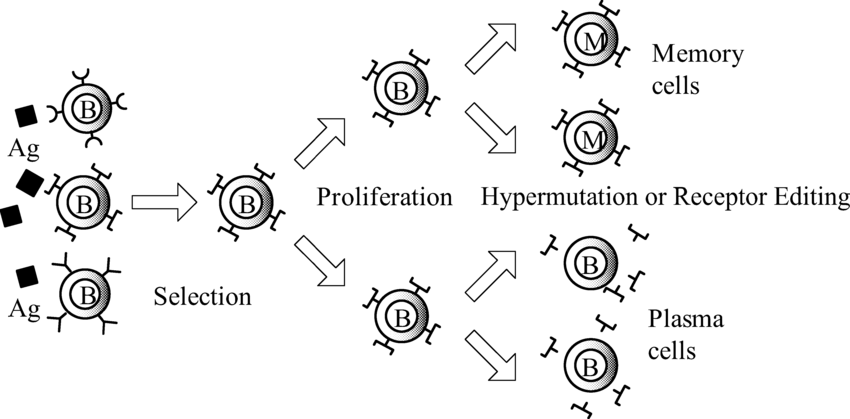
\includegraphics[width=300px]{img/clonal-selection-principle.png}
    \caption{A diagram illustrating the clonal selection process. \cite{Dai07}}
    \label{fig:csp}
\end{figure}

The clonal selection algorithm is inspired by the clonal selection process presented above. While genetic algorithm relies on the evolutionary characteristic of sexual reproduction, clonal selection algorithm relies on the evolutionary characteristic of our immune system. A few best-fit individuals will proliferate, creating the clonal population. This clonal population undergoes hypermutation or receptor editing and the fitness is evaluated again. A few best-fit individuals will be chosen again subsequently to be put in the intermediate population. Until the size of the intermediate population is equal to the desired population size, top individuals from original current population will fill up the remaining intermediate population. This ensures the idea of elitism that best individuals are always preserved without getting lost to mutations. Additionally, a couple random new individuals may occasionally be introduced to the new population.

The main difference between somatic hypermutation and receptor editing is the degree of variation that each brings to a population. Whereas somatic hypermutation is an accumulation of point mutations in B cells, receptor editing is more analgous to chromosomal mutations that involves a long segment of DNA. Consequently, hypermutation usually brings smaller changes to an individual's affinity while receptor editing usually larger changes to the affinity. Hypermutation uses the method of \textit{hillclimbing} to find the solution. In a curve that relates gene expressions and affinity, hillclimbing will either move up or down by a small amount in the curve. The accumulation of hillclimbing will eventually lead to the finding of the hill's local maximum. Receptor editing meanwhile allows us to jump from one hill to another by bringing larger changes, enabling the search for the global maximum. See figure below.

\begin{figure}[H]
    \centering
    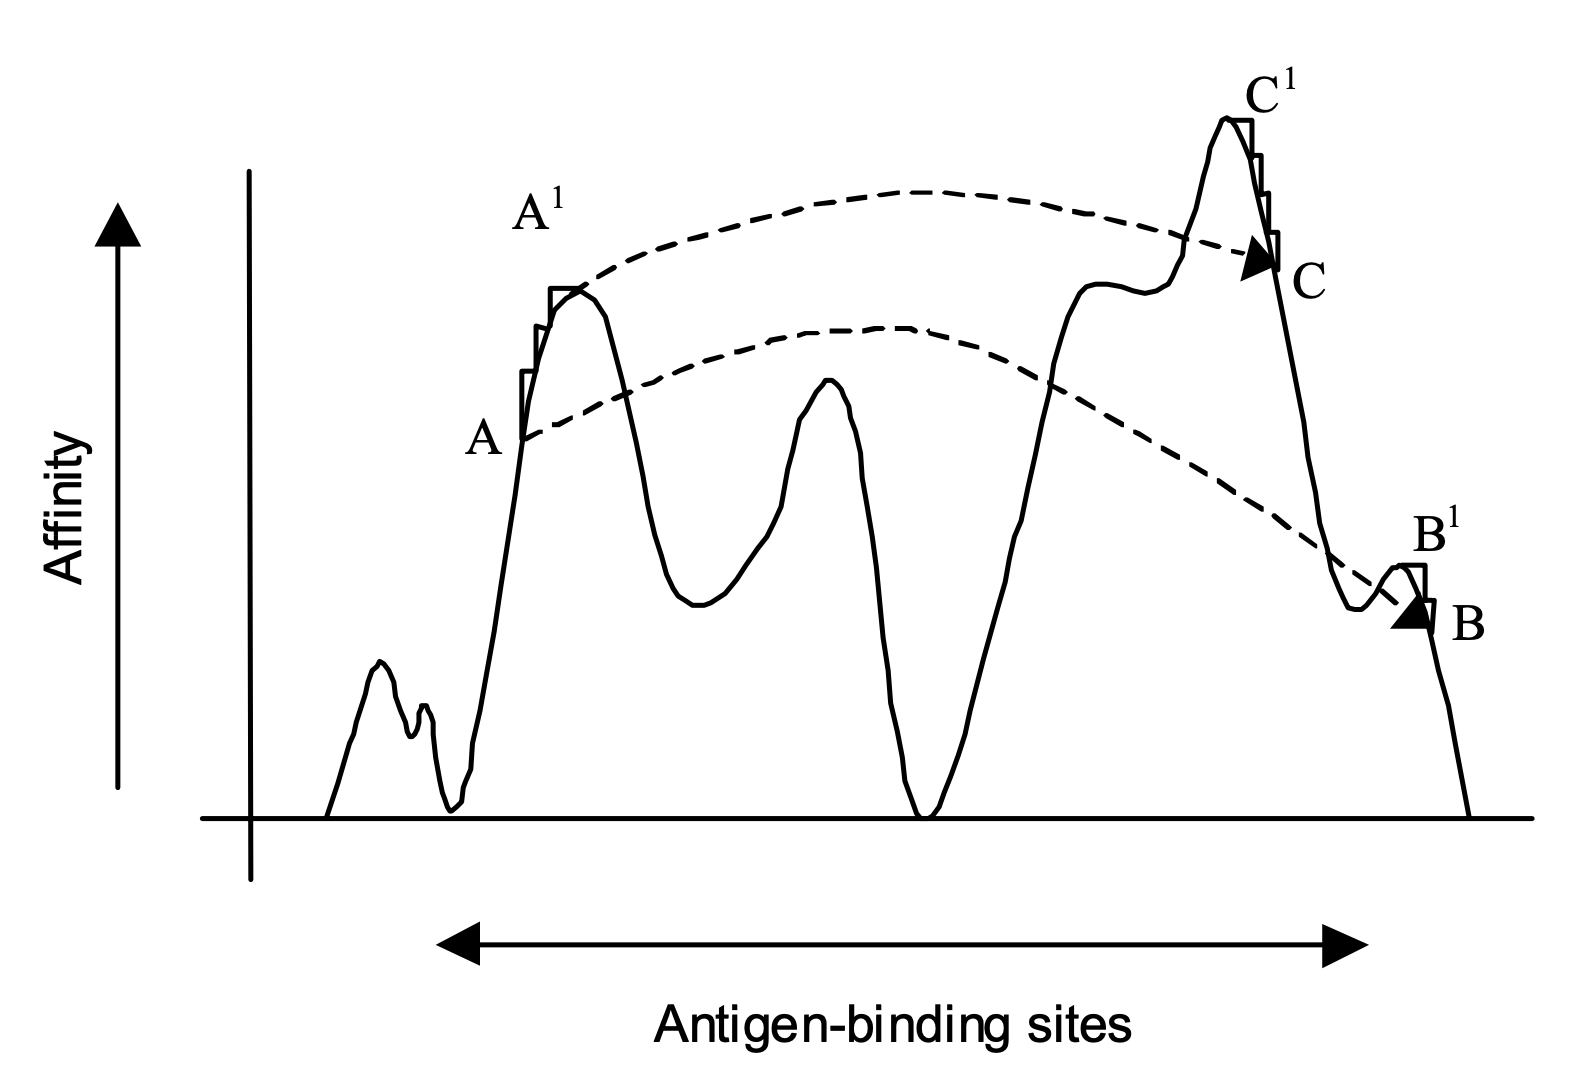
\includegraphics[width=200px]{img/affinity-curve.png}
    \caption{Antigen-binding site-affinity curve. Somatic hypermutation allows the individual at point A to search for the local maximum A' by slowly moving up the hill. Recepting editing allows A to jump to points B or C at different hills and search for the global maximum C'. \cite{Cas01}}
    \label{fig:affinity}
\end{figure}

\subsection{Artificial Neural Network}
Artificial neural network, or ANN, simulates mutual interactions between neurons of an animal's brain to solve complex calculations. Neurons are biological cells present in human brains, and they are composed of parts such as the nucleus, cell body, dendrites, axons, and synaptic terminals. Dendrites receive signals from other neurons, axon conveys signals through the neuron, and synaptic terminals release neurotransmitters and convey them to next neuron in the biological neural network. 

\begin{figure}[H]
    \centering
    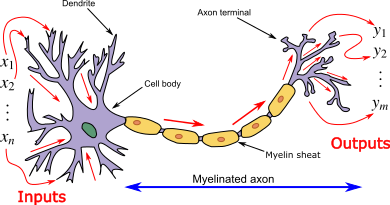
\includegraphics[height=150px]{img/biological-neuron.png}
    \caption{An image of a motor neuron. Inputs are received through the dendrites, and outputs are released by the axon terminals.}
    \label{fig:biological-neuron}
\end{figure}

An artificial neuron is inspired by such interaction of dendrites, an axon, and axon terminals in a biological neuron. Similar to how dendrites receive electric signals and transmit the signal through the axon once the membrane electric potential reaches its critical threshold, an artificial neuron takes in numerical inputs and uses weights and bias to calculate a sum. This sum is ``activated" by some activation function and outputs a final value. Typically, an artificial neural network connects multiple of these artificial neurons and comprises different layers. The three major layers of an artificial neural network are input, hidden, and output layers. Hidden layers can be a set of multiple layers that serve different functions of a problem.

\subsection{The Self-Driving Mechanism}

The simple self-driving car mechanism will take five numerical inputs from the car's raycast sensors that detect a wall. The angle of detection are the five inputs to the input layer, and they are combined with a feed-forward $5 \times 4 \times 3 \times 2$ neural network that determines the car's instantaneous tangential and radial acceleration. The neural network's weights are the genes of our genetic and clonal selection algorithm, whose fitness is eventually determined by the sigmoid function that  recombines the weights into a fitness value between 0 and 1.\footnote{The unity project used in this paper is a modified version of Samuel Arzt's Applying\_EANNs github repository.}

\begin{figure}[H]
\centering
\subfloat[An illustration of car raycast physics in action.]{%
\resizebox*{5cm}{!}{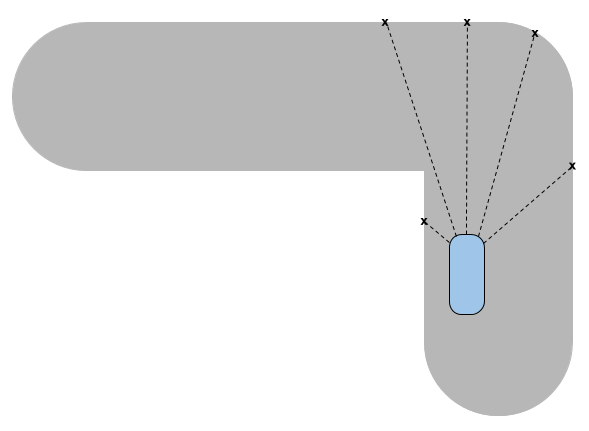
\includegraphics{img/raycast.png}}}\hspace{15pt}
\subfloat[An image of track used.]{%
\resizebox*{7.5cm}{!}{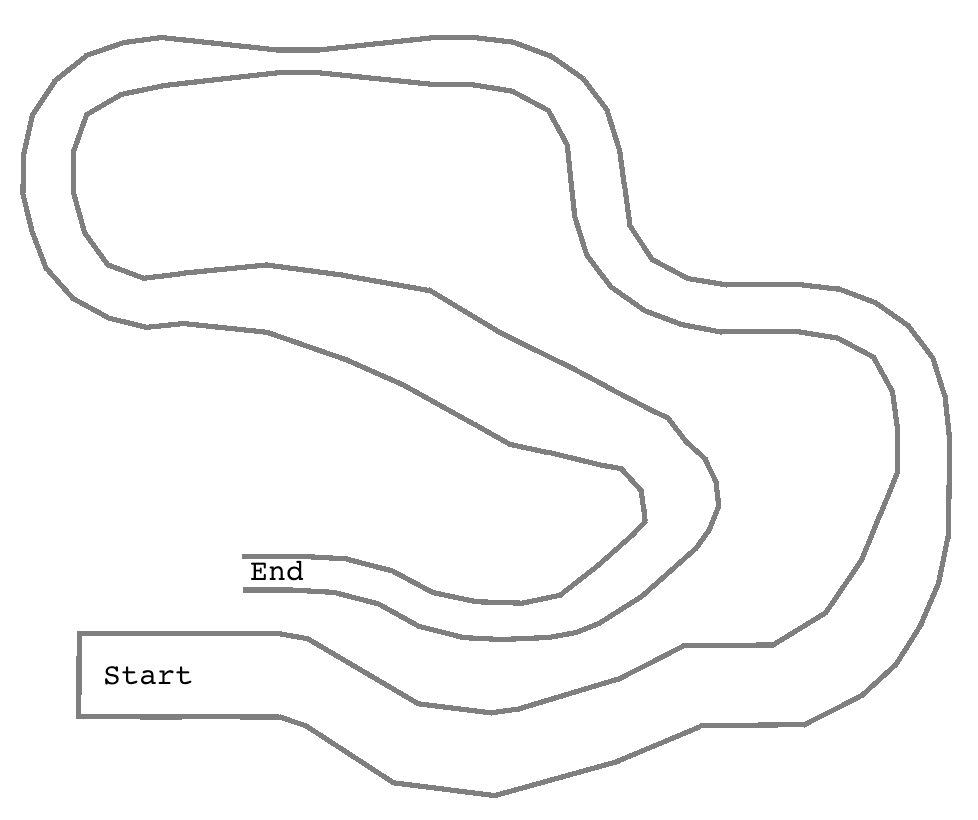
\includegraphics{img/track.png}}}
\label{self-driving}
\caption{Implementation of trivial self-driving methods.}
\end{figure}

\section{Pseudocodes}

\subsection{Roulette Wheel Selection}

\begin{algorithmic}[1]
    \Function{Roulette Wheel Selection}{$currentPopulation$}
    \State $totalSum \leftarrow 0$
    \For{$p_i \in curentPopulation$}
        \State $totalSum \leftarrow totalSum + p_{i}.fitness$
    \EndFor
    \While{$inntermediatePopulation.size < maxPopulationSize$}
        \State Generate $randomDouble$ between 0 and $totalSum$
        \State $prefixSum \leftarrow 0$
        \For{$p_i \in currentPopulation$}
            \State $prefixSum \leftarrow prefixSum + p_i.fitness$
            \If {$randomDouble < prefixSum$}
                \State Add $p_i$ to intermediatePopulation
                \State \textbf{Break}
            \EndIf
        \EndFor
    \EndWhile
    \State \textbf{Return} $intermediatePopulation$
	\EndFunction
\end{algorithmic}

\subsection{Rank Selection}

\begin{algorithmic}[1]
    \Function{Rank Selection}{$currentPopulation$}
        \For{$p_i \in currentPopulation$}
            \State Generate $randomDouble$ between 0 and 1
            \If {$randomDouble < p_i.selectionPercentage$}
                \State Add $p_i$ to intermediatePopulation
                \State \textbf{Break}
            \EndIf
        \EndFor
    \State \textbf{Return} $intermediatePopulation$
	\EndFunction
\end{algorithmic}

\subsection{Remainder Stochastic Sampling}

\begin{algorithmic}[1]
    \Function{Ramainder Stochastic Sampling}{$currentPopulation$}
    \State $averageFitness \leftarrow Sum(currentPopulation) \div populationSize$
    \For{$p_i \in currentPopulation$}
        \State $ratio \leftarrow p_i.fitness \div averageFitness$
        \If{$ratio < 1$}
        \State \textbf{Break}
        \Else
        \State Add $Floor(ratio)$ copies of $p_i$ to $intermediatePopulation$
        \EndIf
    \EndFor
    \For{$p_i \in currentPopulation$}
        \State $ratio \leftarrow p_i.fitness \div averageFitness$
        \State $remainder \leftarrow ratio - Floor(ratio)$
        \State Generate $randomDouble$ between 0 and 1
        \If {$randomDouble < remainder$}
        \State Add $p_i$ to $intermediatePopulation$
        \EndIf
    \EndFor
    \State \textbf{Return} $intermediatePopulation$
	\EndFunction
\end{algorithmic}

\subsection{Clonal Selection \cite{BroND}}

\begin{algorithmic}[1]
    \Function{Clonal Selection Algorithm}{$currentPopulation$}
    \While{$\neg StopCondition()$}
        \For{$p_{i} \in currentPopulation$}
            \State $CalculateFitness(p_{i})$
        \EndFor
        \State Select top few individuals and place in $selectPopulation$
        \For{$p_i \in selectPopulation$}
            \State $clonalPopulation \leftarrow Clone(p_i, numberOfClones)$
        \EndFor
        \For{$p_i \in clonalPopulation$}
            \State $Mutate(p_i, mutationType)$
            \State $CalculateFitness(p_i)$
        \EndFor
        \State Fill $clonalPopulation$ select individuals from $currenPopulation$
        \State Add random individuals to $clonalPopulation$ as desired
        \State $currentPopulation \leftarrow clonalPopulation$
        \State Increment generation count
    \EndWhile
	\EndFunction
\end{algorithmic}

\section{Experiment Design}
A car navigates around the track on roulette wheel selection, rank selection, remainder stochastic sampling, clonal selection with hypermutation, or clonal selection with receptor editing. Each trial is repeated five times. The first three trials for each algorithm records maximum and average fitness of every individuals in a population of each generation. After performing two additional trials, average generation count of the five trials is calculated.

To make the experiment as fair as possible, random generation for initial population is fixed by seeding the random number generator. This allows us to compare how each algorithm evolves at a different pace from equal starting point. Mutation rates are carefully tuned to ensure that the algorithms do not converge too fast, which can lead to finding the local maximum but no global maximum. It is important as well that mutation rates are not too high so that it does not end up becoming a virtual random search. For this problem, it was tuned to a 5\% mutation rate with amount by which numbers may mutate set at 2\%. The population size was set at 30.

\section{Data}

\subsection{Genetic Algorithms: Number of Generations Taken to Complete the Track}
\begin{table}[H]
\centering
\begin{tabular}{c|c|c|c}
Trial   & Roulette Wheel & Rank Selection & Remainder Stochastic Sampling \\ \hline
1       & 22             & 11             & 10                   \\
2       & 38             & 25             & 36                   \\
3       & 32             & 7              & 26                   \\
4       & 21             & 20             & 21                   \\ 
5       & 18             & 24             & 32                   \\ \hline
Average & 26.2           & 17.4           & 25                  
\end{tabular}
\end{table}

\subsection{Clonal Selection Algorithm: Number of Generations Taken to Complete the Track}
\begin{table}[H]
\centering
\begin{tabular}{c|c|c}
Trial   & Hypermutation & Receptor Editing \\ \hline
1       & 10            & 17               \\
2       & 29            & 18               \\
3       & 9             & 16               \\
4       & 8             & 16               \\
5       & 22            & 18               \\ \hline
Average & 15.6          & 17              
\end{tabular}
\end{table}

\subsection{Genetic Algorithm: Graphs Relating Maximum and Average Fitness Over Generations}

\begin{figure}[H]
    \centering
    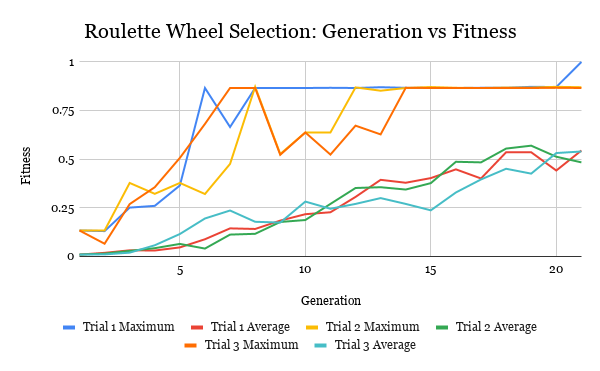
\includegraphics[width=300px]{img/Roulette Wheel Selection_ Generation vs Fitness.png}
    \label{fig:roulette-graph}
\end{figure}

\begin{figure}[H]
    \centering
    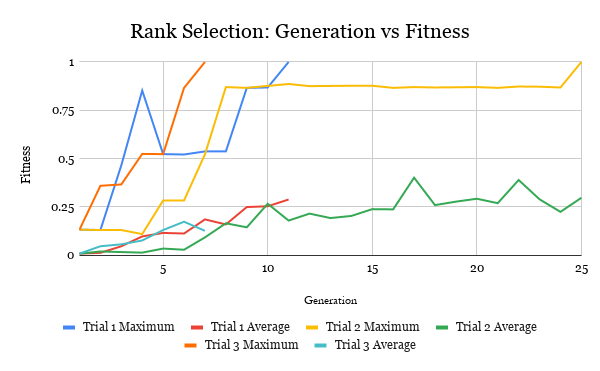
\includegraphics[width=300px]{img/Rank Selection_ Generation vs Fitness.png}
    \label{fig:rank-graph}
\end{figure}

\begin{figure}[H]
    \centering
    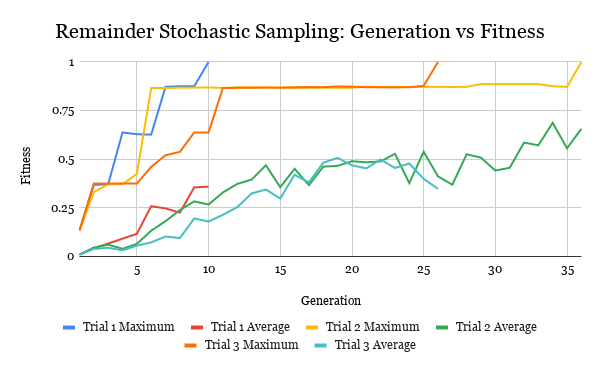
\includegraphics[width=300px]{img/Remainder Stochastic Sampling_ Generation vs Fitness.png}
    \label{fig:remainder-graph}
\end{figure}

\subsection{Clonal Selection Algorithm: Graphs Relating Maximum and Average Fitness Over Generations}

\begin{figure}[H]
    \centering
    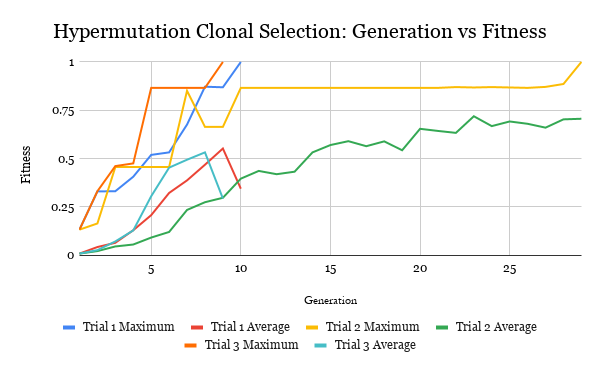
\includegraphics[width=300px]{img/Hypermutation Clonal Selection_ Generation vs Fitness.png}
    \label{fig:hypermutation-graph}
\end{figure}

\begin{figure}[H]
    \centering
    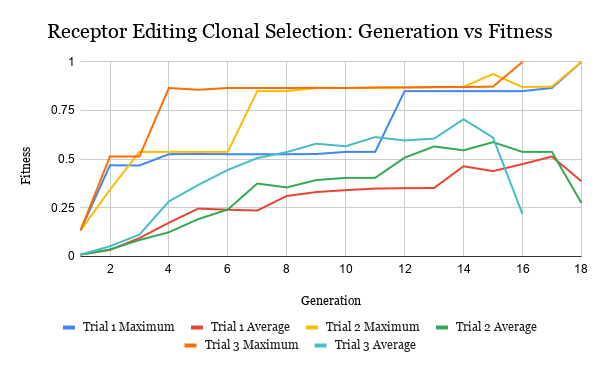
\includegraphics[width=300px]{img/Receptor Editing Clonal Selection_ Generation vs Fitness.png}
    \label{fig:receptor-graph}
\end{figure}

\section{Analysis}

Table 5.1 and 5.2 indicate that rank selection and clonal selection with hypermutation and receptor editing had an average of 17.4, 15.6, and 17 generations, respectively. These averages are significantly less than that of roulette wheel selection and remainder stochastic sampling, which were 26.2 and 25 generations, respectively. One possible explanation for this phenomenon is that top individuals in rank selection and clonal selection have fixed probability of selection whereas roulette wheel selection and remainder stochastic sampling have probability dependent on the fitness of every individual in a population. In other words, selection is absolute in rank and clonal selection and relative in roulette wheel and remainder stochastic sampling. The least-fit individuals in a population are often values random and futile for evolution, and they can lower the chance of selection for top individuals and reapportion that chance to the selection of lesser-fit individuals. Meanwhile, rank selection has a fixed chance of selection for the best-fit individual, which was set at 40\% in this experiment. Clonal selection always selects a certain number of best-fit individuals. This fixed chance independent of lesser-fit individuals' influence ensures elitism and allows the population to evolve from the best ones.

\subsection{Limitations}
One thing to note is that the graphs indicate the evolution of the best-fit individual plateauing around 0.86 until it suddenly discovers an individual of fitness 1.0, which means that the car has completed the track. It was observed that the cars were continuously struggling to successfully maneuver through the sharp curve near the end of the track, which was due to the failure to slow down near the curve and make the turn without collisions. It is rather odd that the raycast physics and the neural network failed to adjust the direction and magnitude of acceleration according to distance and angles. All of the algorithms evolved a gene that reaches the plateau fairly quickly in less than ten generations. It seems more of a matter of suddenly finding a gene that can maneuver through the curve. However, the average fitness shows a steady increase over each generations, which indicates that population is evolving as a whole every time.

\subsection{Somatic Hypermutation vs Receptor Editing}
The average number of generations of each method were similar at 15.6 and 17 generations. However, trials involving hypermutation has a more sporadic set of data while receptor editing has a data set with very low deviation hovering around 17. The best trial for hypermutation took merely 8 generations, but the worst trial took 29. This indicates that receptor editing is more precise and hypermutation is more random. Receptor editing may also hold advantage in a scenario where the fitness of best-individual plateaus because it can quickly jump to the new hills (see Section 2.2) and find a new maximum.

\section{Conclusion and Implication}

\subsection{Benefits of Clonal Selection Algorithm}
The most obvious benefit of an evolutionary algorithm is that it can solve problems that traditional sequential algorithms cannot solve. While standard algorithms may take years and years to solve a NP-complete problem, clonal selection algorithm can quickly discover an approximate solution using nifty evolutionary method. For self-driving, it is nearly impossible to code an algorithm for millions of cases that vehicles may encounter on road. The roads are extremely unpredictable; the cars do not know where and how the curves will turn or when something will suddenly appear. Computer vision can aid this process, but for simple navigation purposes, it will be extremely difficult to code a non-evolutionary algorithm. Clonal selection algorithm was also notably faster than roulette wheel selection and remainder stochastic sampling, which demonstrates the potential of improvements that can be made in this field. Furthermore, its application has immense potential in machine learning as it mimics how our immune system learns through the encounters with pathogens and evolve to ensure the strength of our secondary immune response. 

\subsection{Drawbacks of Clonal Selection Algorithm}
The fundamental problem is the heuristic nature of the algorithm. It may take a very long time to discover a solution or in extremely unlucky circumstances, it may not be able to discover one. This problem becomes more apparent when there is a plateau in the generation-fitness curve because finding a solution then becomes a problem of which individual can mutate into a better individual faster. However, this issue is rather trivial because evolution stems from the idea of natural selection where the best-fit individual survives. The best-fit individual sort of acts as a ``pivot" that prevents the algorithm from turning into a random search, and the drawback is further minimized by ensuring elitism. However, this also requires the meticulous tuning of numbers such as mutation or crossover rates so that the algorithm can converge efficiently.

Most of the drawbacks stem from having suboptimal number of hidden layers, mutation rates, population size, and so on. These values are called hyperparameters because they are set by a user prior to an experiment, unlike parameters such as neural network weights that are learned during the machine learning process. Through hyperparameter optimization techniques, we can minimize the loss function and derive an optimal tuple of hyperparameters for the problem.

\begin{thebibliography}{99}

\bibitem{BroND}
Brownlee, J. (n.d.). Clonal selection algorithm. Retrieved March 17, 2020, from Clever Algorithms: Nature-Inspired Programming Recipes website: http://www.cleveralgor ithms.com/nature-inspired/immune/clonal\_selection\_algorithm.html 

\bibitem{Bus01}
Busetti, F. (2001, May). Genetic algorithms overview. Retrieved from https://ww w.researchgate.net/profile/Franco\_Busetti/publication/2383112\_Genetic\_Algorithms\_Over view/links/5c0e66e592851c39ebe262ca/Genetic-Algorithms-Overview.pdf

\bibitem{Cas01}
Castro, L., \& Zuben, F. (2001, February). The clonal selection algorithm with engineering applications. Retrieved from https://www.researchgate.net/publication/24686 77\_The\_Clonal\_Selection\_Algorithm\_with\_Engineering\_Applications 

\bibitem{CloND}
Clonal selection theory [Image]. (n.d.). Retrieved from https://www.britannica.com/ science/clonal-selection-theory/images-videos

\bibitem{Dai07}
Dai, H., Jianchen, Z., \& Zheng, T. (2007, December). An improved clonal selection algorithm and its application to traveling salesman problems [Image]. Retrieved from https://www.researchgate.net/figure/The-clonal-selection-principle\_fig1\_31492211 

\bibitem{Cas00}
De Castro, Leandro \& José, Fernando \& von Zuben, Antonio Augusto. (2000). Artificial Immune Systems: Part I-Basic Theory and Applications. 

\bibitem{Obi98}
Obitko, M. (1998). Selection. Retrieved March 17, 2020, from Introduction to Genetic Algorithms website: https://obitko.com/tutorials/genetic-algorithms/selection.php

\bibitem{UoA00}
University of Arizona. (2000, November 10). Immunology problem set. Retrieved March 17, 2020, from The Biology Project website: http://www.biology.arizona.edu/immunology /tutorials/immunology/09t.html 

\end{thebibliography}

\end{document}